\section{The basic basics}

\begin{frame}
	\frametitle{About git\footnote{\emph{git} means "unpleasant person" in British slang. Linus: "I'm an egotistical bastard, and I name all my projects after myself."}}
	
	\begin{itemize}
		\item A \emph{distributed} version control system (VCS) 
		\item Developed in 2005 by Linus Torvalds to support Linux kernel development
		\item Git was never meant to be used directly :)
		\item Very powerful and very complex
		\item Supports different workflows
		\item We'll be using the GitHub workflow (more or less)	
	\end{itemize}
	
\end{frame}

% -----------------------------------------------------------------------------

\begin{frame}
	\frametitle{VCS requirements}
	
	\begin{block}{Basic requirements}
	\begin{itemize}
		\item Keep track of changes to our code
		\item Facilitate collaboration
	\end{itemize}
	\end{block}
	
	\begin{block}{Additional requirements}
	\begin{itemize}
		\item Work offline
		\item Support a distributed workflow
		\item Compatibility with existing protocol (e.g. ssh, http)
		\item Cryptographic authentication of history
		\item Efficiency
	\end{itemize}
	\end{block}
\end{frame}

% -----------------------------------------------------------------------------

\begin{frame}[fragile]
	\frametitle{A note on notation}
	
	Throughout the presentation, the following notation applies:
	\begin{itemize}
		\item Commands that you are supposed to type are displayed in \texttt{monospace font} preceeded by a \texttt{>} symbol, such as
		\begin{minted}{console}
		> git --help
		\end{minted}
		\item The \texttt{>} symbol only indicates the command prompt, don't type it in
		\item Text that you need to modify is indicated given \texttt{<inside angle brackets>}, e.g.,
		\begin{minted}{console}
		> cd /home/<your username>
		\end{minted}
		\item Again, when typing the command, omit the brackets
	\end{itemize}
\end{frame}

% -----------------------------------------------------------------------------

\begin{frame}[fragile]
	\frametitle{Getting started: repositories, forking and cloning}

	\begin{block}{Repository (repo)}
	A place where your work is stored. It contains your code and its complete history. 
	\end{block}

	\begin{block}{Forking}
	To fork a repo, simply click the 
\includegraphics[scale=0.35]{fork} icon in the top right corner of the repo webpage. For this tutorial, you will need to clone the \href{https://github.com/larics/git-tutorial}{larics/git-tutorial} repo.
	\end{block}

	\begin{block}{Cloning}
	Cloning creates a local copy of the repository (including \emph{all history}).	
	\begin{minted}{console}
	> git clone git@github.com:<username>/git-tutorial
	\end{minted}
	Clone only one repo per pair!
	\end{block}
\end{frame}
	
% -----------------------------------------------------------------------------

\begin{frame}[fragile]
	\frametitle{Repository structure}
	
	What's in a repository (besides code)?
	
	\begin{minted}{console}
	> cd git-tutorial
	> ls -la
	\end{minted}
	
	The hidden \texttt{.git} folder contains repository metadata (history + internal data structures keeping track of your work).
	
	The \texttt{git status} command provides an overview of what is going on in your repo.
	\begin{minted}{console}
	> git status
	\end{minted}
	
\end{frame}

% -----------------------------------------------------------------------------

\begin{frame}[fragile]
	\frametitle{Changing files and committing your changes}
	
	\begin{block}{Task}
	Open the \texttt{README.md} file and add the following lines, then save the file:
	\begin{minted}{console}
Maintainers:
  <your name>
	\end{minted}
	\end{block}
	
	\begin{minted}{console}
	> git status
	> git diff
	> git add README.md
	> git commit -m "Add maintainer."
	> git status
	\end{minted}

	\begin{block}{Task}
	Use the \texttt{gitg} command to open a GUI and visualize your repo. A similar tool is available on GitHub repository, under the Graphs->Network menu.
	\end{block}
	
\end{frame}

% -----------------------------------------------------------------------------

\begin{frame}[fragile]
	\frametitle{Visualizing git operation}
	
	\begin{figure}
		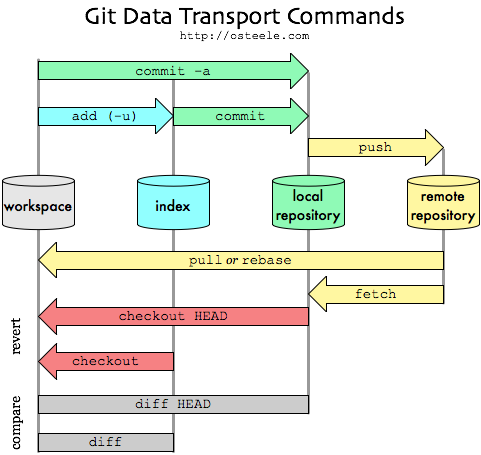
\includegraphics[scale=0.4]{git-transport}
	\end{figure}
\end{frame}

% -----------------------------------------------------------------------------

\begin{frame}[fragile]
	\frametitle{Pushing the changes to the remote repository}
	
	\begin{block}{Local vs. remote changes}
	\texttt{commit} only saves changes \alert{locally}! We need to use \texttt{push} to, well, push the changes to the remote repository. 
	\end{block}
	
	\begin{minted}{console}
	> git push origin master
	\end{minted}
	
\end{frame}

% -----------------------------------------------------------------------------


\begin{frame}[fragile]
	\frametitle{Getting changes from the remote repository}
	
	Getting changes is a two-step process:
	\begin{enumerate}
		\item \texttt{fetch} the changes from the remote repository
		\item \texttt{merge} the changes into your working tree
	\end{enumerate}
	
	\begin{minted}{console}
	> git fetch
	> git status
	> git diff master origin/master
	> git merge origin/master
	\end{minted}
	
	\begin{block}{\texttt{fetch}+\texttt{merge}=\texttt{pull}?}
	\texttt{pull} will do \texttt{fetch} and \texttt{merge} in a single step. However, if \texttt{origin} has changed, you might get yourself into trouble.\footnote{A really nice article advocating the use of \texttt{fetch}+\texttt{merge} can be found on \href{http://longair.net/blog/2009/04/16/git-fetch-and-merge/}{Mark's Blog}} 
	\end{block}
\end{frame}

% -----------------------------------------------------------------------------

\begin{frame}[fragile]
	\frametitle{Discarding unwanted changes}
	
	\begin{block}{Task}
	Make a change to your file. Do not commit.	
	\end{block}
	
	Uncommitted changes can be reverted with \texttt{checkout}:
	\begin{minted}{console}
	> git checkout <yournickname>.md
	\end{minted}
	
	You can also revert to a previous version of a file (an earlier commit)\footnote{now you should start seeing why commit messages are important}:
	\begin{minted}{console}
	> git log --oneline
	> git checkout <commit> <file>
	\end{minted}
	This is the same as making any other change to a file, i.e., it can be committed and pushed.
	% TODO: find out how to discard the change that has been made by the checkout
\end{frame}

% -----------------------------------------------------------------------------

\begin{frame}[fragile]
	\frametitle{Dealing with conflicts (1)}
	
	\begin{block}{Task}
	Work in pairs. Both persons make a change to the same file. One commits and pushes. The other one commits and tries push but fails. He/she needs to fetch + merge first.	
	\end{block}
	
	At other person (not pushed), push fails:
	\begin{minted}{console}
	> git push origin master
	> git fetch
	> git diff master..origin/master
	\end{minted}
	
	\begin{block}{Understanding \texttt{diff}}
	\texttt{git diff a b} shows changes that need to be applied to \texttt{a} to make it the same as \texttt{b}.
	\end{block}
\end{frame}

% -----------------------------------------------------------------------------
\begin{frame}[fragile]
	\frametitle{Dealing with conflicts (2)}
	
	After merging, the file ends up in a conflicted state:
	\begin{minted}{console}
	> git merge origin/master -m "Descriptive message"
	> less <conflicted file>	
	\end{minted}	
	
	Conflict markers inside the file:
	\begin{minted}{console}
	<<<<<<< HEAD
	Code on working branch before the merge
	=======
	Code introduced by the merge
	>>>>>>> origin/master
	\end{minted}

	To resolve the conflict, manually edit the file, mark resolution by \texttt{git add} commit and push:
	\begin{minted}{console}
	> git commit -am "Resolved conflict..."
	> git push origin master
	\end{minted}
	
\end{frame}

% -----------------------------------------------------------------------------



\begin{frame}[fragile]
	\frametitle{Manipulating files}
	
	Newly created files have to be added to git explicitly:
	\begin{minted}{console}
	> mkdir <myname>
	> echo blabla > <myname>/newfile.md
	> git add <myname>/newfile.md
	\end{minted}
	
	When moving files, you have to tell git about it:
	\begin{minted}{console}
	> git mv <myname>.md <myname>
	> git commit -am "Added, moved..."	
	\end{minted}
	
	Same goes for deleting files:
	\begin{minted}{console}
	> git rm myname/myname.md
	> git commit -am "Removed..."
	\end{minted}
	
	\begin{minted}{console}
	
	\end{minted}
	
\end{frame}

% -----------------------------------------------------------------------------

\begin{frame}[fragile]
	\frametitle{Handling binary files}
	
	\begin{block}{Difference between text and binary files}
	Changes to text files are stored incrementally, as diffs, which is very space-efficient. For every change in a binary file, the whole file is stored again. The change persists, even after the file is removed!
	\end{block}
	
	\begin{block}{How to handle binary files}
	Storing binary files is ok if they are small and change infrequently. Otherwise, create a README file with instructions for downloading the files (or a download script, if you want to be fancy).
	\end{block}
	
	\begin{block}{Build output}
	\alert{Never} commit build output (even if it is text, e.g. documentation)!
	\end{block}
\end{frame}